%%%%%%%%%%%%%%%%%%%%%%%%%%%%%%%%%%%%%%%%%%%%%%%%%%%%%%%%%%%%%%%%
\section{Pendulum Model Variants}
\label{sec:case_study_pendulum_models}

The controlled-pendulum case study uses several plant models behind the shared interface defined in Section~\ref{sec:case_study_controlled_pendulum_system}.
All variants implement this port-level contract.
They differ in modeling approach, internal state, contact representation, and computational cost.

Chapter~\ref{chap:theoretical_background} introduced the modeling approaches and used the pendulum as a running example.
The Modelica realization and the \ac{FMI} translation path were already discussed in Section~\ref{sec:241_modeling_equation_based}.
The OpenSim and \ac{FEM} concepts were introduced in Sections~\ref{sec:242_modeling_musculoskeletal} and~\ref{sec:243_modeling_fem}.
The present section therefore focuses on the concrete case-study variants and on their role in the closed-loop simulations.

Table~\ref{tab:case_pendulum_variants} summarizes the four plant variants.
The \ac{FMU}, OpenSim, and \ac{FEM} variants are individual plant models.
The \texttt{MasterPendulum} wraps these variants and selects the active model during runtime.

\begin{table}[tbp]
  \centering
  \small
  \caption[Pendulum model variants]{Pendulum model variants used in the controlled-pendulum case study.}
  \label{tab:case_pendulum_variants}
  \begin{tabular}{p{3.1cm}p{3.4cm}p{4.3cm}p{3.7cm}}
    \toprule
    \textbf{Variant} & \textbf{Modeling approach} & \textbf{Role in the case study} & \textbf{Main limitation} \\
    \midrule
    \ac{FMU} pendulum
      & Equation-based rigid-body model
      & Efficient baseline plant and low-cost model for switching
      & No spatial deformation or contact field \\
    \addlinespace
    OpenSim pendulum
      & Multibody model
      & Intermediate plant model and tool-integration path
      & No deformable-body contact field \\
    \addlinespace
    \ac{FEM} pendulum
      & Spatially resolved deformable model
      & High-fidelity model for contact-relevant phases
      & Higher computational cost \\
    \addlinespace
    \texttt{MasterPendulum}
      & Multi-model wrapper
      & Runtime switching between plant variants
      & State projection between models of different fidelity \\
    \bottomrule
  \end{tabular}
\end{table}

%%%%%%%%%%%%%%%%%%%%%%%%%%%%%%%%%%%%%%%%%%%%
\subsection{FMU Pendulum}
\label{sec:case_study_pendulum_fmu}

The \ac{FMU} pendulum is the equation-based rigid-body variant of the pendulum.
It is generated from the Modelica pendulum model and exported as an \ac{FMI} 2.0 Co-Simulation unit.
Its state is described by the angle \(\theta\) and angular velocity \(\omega\).
The actuator torque \(\tau\) enters as the external input.
The reported scenarios use the \ac{CVODE}-based \ac{FMU} variant unless stated otherwise~\cite{openmodelica_users_guide_2026}.

This model is used as the low-cost plant representation.
It is the main plant model in the baseline scenario of Section~\ref{sec:case_study_baseline}.
It is also used by the \texttt{MasterPendulum} when the pendulum is far from the contact region.
Because it follows the same lumped rigid-body dynamics as the OpenModelica reference, the baseline comparison mainly exposes the effect of co-simulation coupling and macro-step size.

The \ac{FMU} pendulum is a rigid-body model.
A contact-capable variant represents wall contact through signal-level event handling.
It reacts to a wall event by inverting the angular velocity.
This gives an ideal rigid-impact reference behavior.
Compliant penetration and spatial contact effects are assigned to the \ac{FEM} pendulum.

%%%%%%%%%%%%%%%%%%%%%%%%%%%%%%%%%%%%%%%%%%%%
\subsection{OpenSim Pendulum}
\label{sec:case_study_pendulum_opensim}

The OpenSim pendulum represents the same one-degree-of-freedom plant as an articulated multibody model.
It consists of a fixed base, a pendulum body, and a pin joint with generalized coordinate \(\theta\).
A \texttt{CoordinateActuator} applies the input torque \(\tau\) at the joint.
The outputs \(\theta\) and \(\omega\) are read from the generalized coordinate and speed.
Both quantities are state variables of the OpenSim model.

The OpenSim variant is included as the domain-specific multibody tool path of the case study.
The OpenSim variant uses a passive pin-joint model without muscle dynamics.
This keeps the OpenSim model comparable to the \ac{FMU} pendulum and focuses the comparison on tool integration and model interchangeability.
The model therefore uses the same shared plant interface as the other pendulum variants.

The physical parameters of the OpenSim pendulum are synchronized from the \ac{FEM} pendulum when it is used inside the \texttt{MasterPendulum}.
The synchronized quantities are the total mass, the center-of-mass length, and the moment of inertia about the pivot.
The OpenSim body inertia is then chosen so that the parallel-axis relation gives the same pivot inertia.
This avoids switching between pendulum variants that represent different rigid-body dynamics.

In the multi-model scenario, the OpenSim pendulum acts as an intermediate-fidelity plant model.
It is used between the low-cost \ac{FMU} region and the contact-relevant \ac{FEM} region.
It does not resolve deformable contact or local stress fields.
Those effects are assigned to the \ac{FEM} pendulum.

%%%%%%%%%%%%%%%%%%%%%%%%%%%%%%%%%%%%%%%%%%%%
\subsection{FEM Pendulum}
\label{sec:case_study_pendulum_fem}

The \ac{FEM} pendulum is the high-fidelity pendulum variant of the case study.
It replaces the lumped rigid body by a spatially resolved deformable body.
It is used when the pendulum approaches the wall and when the contact response must be resolved.
The general finite element theory was introduced in Section~\ref{sec:243_modeling_fem}.
This subsection only describes the case-study-specific realization.

\paragraph{Geometry and material.}
The model is a thin two-dimensional pendulum under a plane-stress assumption.
The geometry consists of a narrow rod and a circular head.
The circular head contains the contact boundary.
The lower edge at the pivot is named the rotation boundary.
When contact is enabled, the wall is included as a second finite element body.
Its outer boundaries are fixed, while the wall-side contact edge is paired with the pendulum head.

The reported contact scenarios use the Saint Venant--Kirchhoff material law with steel-like parameters.
The implementation also supports a Neo-Hookean law through the same component interface.
The Young's modulus, Poisson ratio, density, thickness, and contact stiffness are stated with the scenario parameters in Section~\ref{sec:case_study_multimodel_contact}.
This keeps the model description separate from the numerical comparison.

Figure~\ref{fig:case_fem_model} gives the geometric and field context for the \ac{FEM} variant.
It identifies the mesh, material domains, and boundary regions used by the model.
The stress panel illustrates that the \ac{FEM} component contains spatial field quantities, although the co-simulation interface exposes only the projected angle and angular velocity.

\begin{figure}[t]
  \centering
  \begin{subfigure}[t]{0.45\textwidth}
    \centering
    
\includegraphics[width=\linewidth]{figures/6_case_study/controlled_pendulum/fem_mesh_boundaries.pdf}
    \caption{Reference mesh and boundary regions.}
  \end{subfigure}
  \hfill
  \begin{subfigure}[t]{0.45\textwidth}
    \centering
    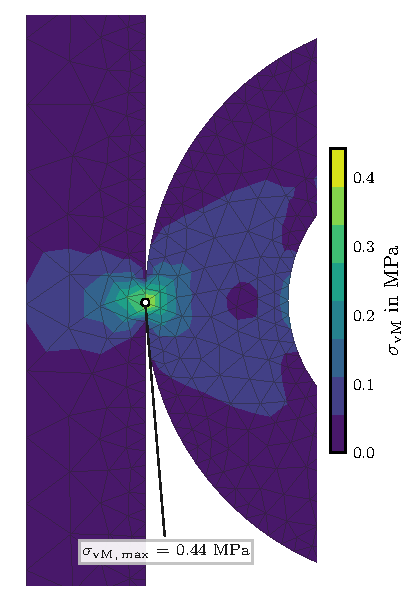
\includegraphics[width=\linewidth]{figures/6_case_study/controlled_pendulum/fem_deformed_contact_von_mises_zoom.pdf}
    \caption{Contact stress field.}
  \end{subfigure}
  \caption[\ac{FEM} pendulum model used for the contact-capable plant variant]{\ac{FEM} pendulum model used for the contact-capable plant variant.
  Panel~(a) shows the reference mesh with the pendulum and wall domains and the boundary regions used for hinge constraint, torque loading, wall contact, and wall fixation.
  Panel~(b) shows a representative von Mises stress field during a free-swing contact run from \(\theta_0=0.30\,\mathrm{rad}\) with gravity and zero drive torque.
  The stress field illustrates the spatial information available inside the \ac{FEM} model.
  No experimental stress validation is claimed.}
  \label{fig:case_fem_model}
\end{figure}

\paragraph{Pivot constraint.}
The pivot is not modeled as a rigid revolute joint.
Instead, the \ac{FEM} model uses a hinge-like constraint on the rotation boundary.
A mixed finite element space augments the displacement field with two scalar Lagrange multipliers.
They enforce zero mean displacement of the rotation boundary in the two Cartesian directions.
This removes rigid translation of the hinge edge while leaving the body free to rotate and deform.

\[
  \int_{\Gamma_{\mathrm{rot}}} \mathbf{u} \,\mathrm{d}s = \mathbf{0}
\]

This is an approximation of an ideal hinge.
It is sufficient for the case study because the surrounding system only observes the projected angular motion of the pendulum.
The local deformation near the hinge remains part of the \ac{FEM} solution.

\paragraph{Time integration.}
The \ac{FEM} state consists of displacement, velocity, and acceleration fields.
The fields are advanced with a Newmark-type time discretization.
At each internal \ac{FEM} step, the nonlinear residual is solved by Newton iteration.
After the displacement solve, the velocity and acceleration fields are updated from the Newmark relations.
The component stores the full integration state so that the hybrid algorithm can take snapshots and restore them during event localization.

The \ac{FEM} time step is internal to the component.
It can be smaller than the macro communication step of the co-simulation.
Near contact, the implementation reduces the internal step size when the contact gap becomes small.
This resolves contact onset and rebound more finely than the surrounding macro step.

\paragraph{Torque boundary.}
The controller and drive provide a scalar torque \(\tau\).
The \ac{FEM} model maps this scalar input to a distributed traction on the rotation boundary.
The traction distribution has approximately zero resultant force and a resultant moment equal to the requested drive torque.

\[
  \int_{\Gamma_{\mathrm{rot}}} \mathbf{t}_{\tau} \,\mathrm{d}s \approx \mathbf{0}
  \qquad
  \int_{\Gamma_{\mathrm{rot}}} \mathbf{r} \times \mathbf{t}_{\tau} \,\mathrm{d}s = \tau
\]

The implementation precomputes an effective moment arm for this mapping.
The traction is applied as a follower load on the current boundary configuration.
This makes the \ac{FEM} input comparable to the torque input of the rigid-body variants while avoiding an artificial net force at the hinge.

\paragraph{Compliant contact boundary.}
Contact is represented by a penalty contribution between the wall boundary and the pendulum head boundary.
The signed gap is evaluated on the current deformed configuration.
When the gap indicates penetration, a contact energy proportional to the square of the penetration measure is activated.
The coefficient \(k_n\) is the normal contact stiffness.

A large value of \(k_n\) makes the contact response stiff and approximates an ideal rigid impact.
The response is still compliant.
Small penetration and phase differences relative to a rigid-contact reference are therefore expected.
This distinction is important for the interpretation of Section~\ref{sec:case_study_multimodel_contact}.
The comparison is limited to a numerical check against a rigid-contact reference.
Physical validation of the contact law would require experimental contact data.

The contact gap is also used as an event indicator.
If the internally stepped \ac{FEM} solution detects a zero crossing of the gap between two internal time points, the component reports an internal event bracket.
The hybrid algorithm can then localize the wall-contact event inside the macro interval.

\paragraph{Output projection.}
The finite element model resolves displacement and velocity fields, but the surrounding co-simulation consumes the shared plant outputs.
The \ac{FEM} component therefore projects these fields onto rigid-body proxy quantities.
The angle \(\theta\) is obtained from a mass-weighted rigid-rotation projection.
The angular velocity \(\omega\) is obtained from the corresponding projected velocity field.

This projection makes the \ac{FEM} pendulum compatible with the shared plant interface.
It also defines the information that is available when the \texttt{MasterPendulum} switches from the \ac{FEM} model to a rigid-body model.
Local deformation and stress fields are not transferred to the lower-fidelity variants.
This is a modeling consequence of runtime model switching between different fidelity levels and is discussed with the results in Section~\ref{sec:case_study_discussion}.

%%%%%%%%%%%%%%%%%%%%%%%%%%%%%%%%%%%%%%%%%%%%
\subsection{Master-Pendulum Wrapper}
\label{sec:case_study_master_pendulum}

The \texttt{MasterPendulum} wraps the \ac{FMU}, OpenSim, and \ac{FEM} pendulum variants behind the shared plant interface of Section~\ref{sec:case_study_controlled_pendulum_system}.
The surrounding closed-loop system therefore connects to one plant component only.
Internally, the wrapper forwards inputs, outputs, and stepping calls to the currently active model.
The implementation details of the underlying \texttt{MultiComponent} abstraction were described in Section~\ref{sec:impl_multi_model}.

The \ac{FEM} pendulum is initialized first because it computes the geometry-dependent reference quantities of the plant.
These quantities are the total mass, the center-of-mass length, and the moment of inertia about the pivot.
The same values are then copied to the \ac{FMU} and OpenSim pendulums.
For OpenSim, the body inertia is chosen so that the parallel-axis relation gives the same pivot inertia.
This synchronization ensures that all variants represent the same nominal pendulum before runtime switching is evaluated.

The switching rule selects the model according to the distance from the contact region.
The \ac{FMU} is used far from contact.
OpenSim is used in the intermediate region.
The \ac{FEM} pendulum is used close to contact.
In the contact scenario, this rule is implemented through thresholds on the absolute pendulum angle and stabilized by hysteresis.
At each switch, the wrapper transfers the shared rigid-body state consisting of \(\theta\), \(\omega\), and \(\tau\).
For the \ac{FMU}, \(\theta\) and \(\omega\) are written as initial-condition parameters because the \ac{FMU} solver state is reset through that interface.
When switching away from \ac{FEM}, the deformable state is projected to these rigid-body quantities.
Local deformation and stress states are not transferred to the lower-fidelity models.
